   \subsection{Generative model}
\label{generativeModel}
    In topic modeling every document viewed as a mixture of topics. Each topic is a multinomial distribution on words,
    so generation model may be defined as follows:
    \begin{itemize} \label{generation}
	\item For every position in document $d$ i.i.d choose topic $t$ from distribution of topics by document
	\item Choose word $w$ from topic $t$
    \end{itemize}
    \begin{figure}[!ht]
	\caption{Graphical representation of PLSA generative process}
	\begin{minipage}{\textwidth}
	    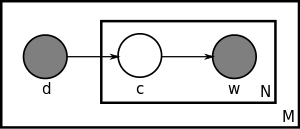
\includegraphics[width=0.55\linewidth]{plsa}
	\end{minipage}
    \end{figure}
    The aim of topic modeling is to recover topics and distribution of every document by topics.
    \subsubsection{Polylingual topic model}
	Suppose one has a collection of documents in different languages. We have a prior knowledge that some of the
	documents (or all of them) are written on the same topic but in different languages (for example one document may be a translation of another).
	Wikipedia may be considered as a source of this type of data. It leads us to a polylingual topic modeling \cite{polylingual}.
	In this model we assume that every topic is a set of multinomial distributions, one per language. Also we assume that
	every document may hold more than one set of words, so we represent document as a map from attributes $\to$  sequences of words.

    \subsubsection{Robust PLSA}
	In robust PLSA we assume that some words are too specific for a document and can not be explained by topic
	distribution. Conversely, some of words are too common and may be explained by any topic.
	Robust PLSA take it into account. In robust PLSA a word may be generated from topic, noise or background.
	Noise is a multinomial distribution over rare words. Every document has its own noise.
	Background is a multinomial distribution over common words. Background is the same for every document.
	To generate words $w$  in document $d$ we:
	\begin{itemize}
	    \item with probability $\propto \gamma$ generate word from noise
	    \item with probability $\propto \varepsilon$ generate word from background
	    \item with probability $\propto 1 - \gamma - \varepsilon$ generate word from topic
		distribution as in \ref{generation}
	\end{itemize}
	$\gamma$ and $\varepsilon$ are hyperparameters of the model.

    \subsubsection{Sparse PLSA} \label{sparseModel} 
	A single document often corresponds to only a few topics, not to every. Analogously,
	word may corresponds only to a few topics, not to every topic. Sparse PLSA takes it into account,
	and replaces some of topics weights in document by zero and replaces some weights in distribution
	of words by topic by zero. Sparsification of topic modeling has some features which allow to sparse distribution of
	words by topic and distribution of document by topics without decreasing of model quality.

    \subsubsection{LDA} \label{LDA}
	LDA is an extension of PLSA, LDA was described in \cite{LDA} and now it is one of the most popular (may be the most popular) topic model. The idea of this model is that
	distribution of documents by topics and distribution of words by topics has Dirichlet \footnote{\url{http://en.wikipedia.org/wiki/Dirichlet_distribution}} (usually, symmetric) prior distribution and we maximize marginal distribution $P(data, parameters)$ instead of conditional one \-- $P(data | parameters)$. 
	\begin{figure}[!ht]
	\caption{Graphical representation of LDA generative process}
	\begin{minipage}{\textwidth}
	    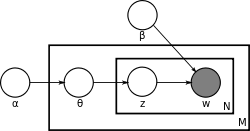
\includegraphics[width=0.55\linewidth]{lda}
	\end{minipage}
	\end{figure}\\
	$\alpha$ and $\beta$ are hyperparameters of the model. 
 
    \subsection{Topic modeling as optimization problem}
	According to generative model one can estimate probability to observe collection $D$ as:
	\begin{equation} p(D) = \prod_{d \in D} \prod_{w \in d} \sum_{t} p(t|d) p(w|t) \end{equation}
	Denote $\varphi_{wt} = p(w|t)$ and $\theta_{td} = p(t|d)$. One can obtain $\varphi_{wt}$
	and $\theta_{td}$ as a solution of optimization problem

	\begin{equation} \label{optimization} L = \sum_{d \in D} \sum_{w \in d} \log \sum_{t} \varphi_{wt} \theta_{td}  \to \max \end{equation}
	    with boundaries
	\begin{equation} \forall t \ \ \sum_{w} \varphi_{wt} = 1, \ \ \forall d \ \ \sum_{w} \theta_{td} = 1 \end{equation}
	and
	\begin{equation} \forall t, w \ \  \varphi_{wt}  \geq 0, \ \ \forall d, t \ \ \theta_{wt}  \geq 0 \end{equation}

    \subsection{Topic modeling as matrix decomposition} \label{matrixDecomposition}

	\subsubsection{Kullback-Leibler divergence}
	    Kullback-Leibler divergence is a non-negative semi-metric between a pair of probability distributions:
	    \begin{equation} KL(p_i||q_i) = \sum_{i=1}^n p_i \ln\left(\frac{p_i}{q_i}\right)  \end{equation}
	    Consider an empirical distribution $\hat{p}_i$ and some parametric distribution $q_i = q_i(\alpha)$ which is used to explain $\hat{p}_i$ .
	    Easy to see that in this case minimization of KL\---divergence is equivalent to estimation of $\alpha$ by maximum-likelihood:
	    \begin{equation} KL(p_i||q_i(\alpha)) = \sum_{i=1}^n p_i \ln\left(\frac{p_i}{q_i(\alpha)}\right) \to \min_{\alpha}
	    \Leftrightarrow \sum_{i=1}^n p_i \ln(q_i(\alpha)) \to \max_{\alpha} \end{equation}

	    Thus one can easily see that (\ref{optimization}) equivalent to weighted Kullback-Leibler divergence minimization:
	    \begin{equation}
		\sum_{d \in D} n_d KL_w \left( \frac{n_{dw}}{n_d} || \sum_{t \in T} \varphi_{wt}\theta_{td} \right) \to \min_{\Phi, \Theta}
	    \end{equation}
		where $n_{wd}$\--- number of words $w$ in document $d$, $n_d$ \--- number of words in document $d$.

	\subsubsection{Matrix decomposition}
	    Denote empirical distribution of words by document as $\hat{p}(w, d) = \frac{n_{wd}}{n_d}$.
	    According to this notation one can consider the problem (\ref{optimization}) as matrix decomposition:
	    \begin{equation} F \approx_{KL} \Phi \Theta \end{equation}
	    where matrix $F = (\hat{p}(w, d))_{W \times D}$ is empirical distribution of words by document,
	    matrix $\Phi = (\varphi_{wt})_{W \times D}$ is distribution of words by topics and
	    matrix  $\Theta = (\theta_{td})_{T\times D}$ is distribution of documents by topics.
	    Thus, our optimization problem may be rewritten in Kullback–Leibler notation as
	    \begin{equation} KL(F , \Phi \Theta) \rightarrow \min \end{equation}
	    Thus PLSA may be observed as stochastic matrix decomposition.

    \subsection{Expectation\--Maximization algorithm} \label{EMAlgorithm}
	    Unfortunately (\ref{optimization}) has no analytical solution. Thus we use Expectation \-- Maximization (EM) algorithm.
	    This algorithm consists of two steps:
	    \begin{enumerate}
		\item Estimation of number $n_{dwt}$ of words $w$, produced by topic $t$ in document $d$. (E \-- step)
		\item Optimization of distribution of documents by topics and optimization of distribution of topics by words relying on
		    the $n_{dwt}$ values obtained during E \-- step . (M \-- step)
	    \end{enumerate}
	    One can estimate $n_{dwt}$ as follows:
	    \begin{equation}  n_{dwt} = n_{wd} p(w|t) p(t|d) \end{equation}
	    where $n_{wd}$ \--- number of words $w$ in document $d$.
	    Thus, probability $p(w|t)$ may be estimated as
	    \begin{equation}  p(w|t) = \frac{n_{wt}}{n_t} = \frac{\sum_d n_{dwt} }{\sum_w \sum_d n_{dwt}}   \end{equation}
	    Similarly for $p(t|d)$

	\subsubsection{Complexity}
	Obviously, time complexity for every iteration is $O(T \times n_{uniq} \times D)$.\\
	Space complexity is given by $O(W \times T + D \times T)$.\\
	Here $n_{uniq}$ is the average number of distinct tokens in a document, $D$ stands for number of documents and $W$  -- for the size of vocabulary.

    \subsection{Regularizers} \label{Regularizers}
	Regularizers may improve human-understandability of the topics, transform PLSA to LDA, provide an ability
	for semi-supervised learning (employ a prior knowledge about document topic or topics structure), select number of topics.
	Instead of optimization (\ref{optimization}) we optimize
	\begin{equation} \label{optimizeWithReqularizer} L(\Phi, \Theta) + R(\Phi, \Theta) \to \max_{\Phi, \Theta} \end{equation}
	Where $R(\Phi, \Theta)$ is a twice differentiable function, named regularizer.
	Solution of this problem leads to a modification of M\--step:
	\begin{equation}
	    \label{RegularizersEquation}
	    \varphi_{wt} \propto \left(\hat{n}_{wt} + \varphi_{wt} \frac{\partial  R(\Phi, \Theta)}{\partial \varphi_{wt}} \right)_+ ,\ \
	    \theta_{td} \propto \left(\hat{n}_{dt} + \theta_{td}\frac{\partial  R(\Phi, \Theta)}{\partial \theta_{td}} \right)_+
	\end{equation}
	Where $\hat{n}$ has been estimated by E\--step.

	\subsubsection{Probability interpretation}
	    Does regularizer have probabilistic interpretation? Yes, it does. Imagine that $\Phi$ and $\Theta$ have some prior distribution, for example
	    dirichlet distribution. In this case:
	    \begin{equation} \label{probabilityWithReqularizer} P(D, \Theta, \Phi) = P(D| \Theta, \Phi) \times P(\Theta, \Phi) \end{equation}
	    Take the logarithm of the equation \ref{probabilityWithReqularizer}:
	    \begin{equation} \ln P(D, \Theta, \Phi) = \ln(P(D| \Theta, \Phi) \times P(\Theta, \Phi) = \ln(P(D| \Theta, \Phi)) + \ln(P(\Theta, \Phi)) \end{equation}
	    Denote $L(\Phi, \Theta) = \ln(P(D| \Theta, \Phi))$ and $R(\Phi, \Theta) = \ln(P(\Theta, \Phi))$ and obtain \ref{optimizeWithReqularizer}

	    \paragraph{Example}
		Consider the example with symmetric dirichlet distribution\footnote{\url{http://en.wikipedia.org/wiki/Dirichlet_distribution}} with parameter $\alpha$.
		Assume we estimate $n_{td}$ for each topic in E\--step and want to perform M\-- step. We would find new distribution of document by topic as a maximum posterior probability solution:
		\begin{equation} \ln(P(\vec{\theta}| \vec{n}_{dt})) \to \max \end{equation}
		\begin{equation} \ln(P(\vec{\theta}| \vec{n}_{dt})) \propto \ln(P(\vec{n}_{dt}|\vec{\theta}) \times P(\vec{\theta})) \Leftrightarrow \end{equation}
		\begin{equation} \ln(P(\vec{\theta}| \vec{n}_{dt})) = \ln(\prod_{t \in T} \theta_t^{n_{td}} \times \prod_{t \in T}\theta_t^{\alpha - 1}) + const \Leftrightarrow  \end{equation}
		\begin{equation} \label{regularizerEquation} \ln(P(\vec{\theta}| \vec{n}_{dt})) = (\sum_{t \in T}(n_{td} + \alpha - 1) \ln(\theta_t)  + const \Leftrightarrow  \end{equation}
		And boundary:
		\begin{equation} \label{regularizerBoundary} \sum_{t \in T} \theta_t = 1 \end{equation}
		We may write down a Lagrangian from \ref{regularizerEquation} and \ref{regularizerBoundary}
		\begin{equation} L(\vec{\theta}, \lambda) = \sum_{t \in T}(n_{td} + \alpha - 1) \ln(\theta_t) - \lambda (\sum_{t \in T} \theta_t - 1)  \end{equation}
		\begin{equation} \frac{\partial L}{\partial \theta_t} = \frac{n_{td} + \alpha - 1}{\theta_t} - \lambda = 0  \end{equation}
		\begin{equation} \theta_t \propto  n_{td} + \alpha - 1 \end{equation}
		Where $n_{td}$ was estimated in E\--step and
		$\theta_{td}\frac{\partial  R(\Phi, \Theta)}{\partial \theta_{td}} = \theta_{td} \frac{\partial (\alpha - 1)\ln(\theta_{td})}{\partial \theta_{td}} = \alpha - 1 $
		is regularizer.\\
		See example of regularizer implementation in ru.ispras.modis.tm.regularizer.SymmetricDirichlet
		
		